\documentclass{article}[a4paper]
\usepackage[utf8]{inputenc}
\usepackage[spanish]{babel}
\usepackage[a4paper, 11pt]{geometry}
\usepackage{graphicx}
\newcommand{\xor}{\oplus}
\usepackage{xcolor}
\usepackage{listings} %code highlighter
\usepackage{blindtext}
\usepackage{titlesec}
\usepackage{appendix}
\usepackage[T1]{fontenc}
\usepackage{textcomp}
\usepackage{amssymb,amsmath}
\usepackage{hyperref}

\newcommand\tab[1][1cm]{\hspace*{#1}}

\definecolor{codegreen}{rgb}{0,0.6,0}
\definecolor{codegray}{rgb}{0.5,0.5,0.5}
\definecolor{codepurple}{rgb}{0.58,0,0.82}
\definecolor{backcolour}{rgb}{0.95,0.95,0.92}

\lstdefinestyle{mystyle}{
    backgroundcolor=\color{backcolour},   
    commentstyle=\color{codegreen},
    keywordstyle=\color{magenta},
    numberstyle=\tiny\color{codegray},
    stringstyle=\color{codepurple},
    basicstyle=\ttfamily\footnotesize,
    breakatwhitespace=false,         
    breaklines=true,                 
    captionpos=b,                    
    keepspaces=true,                 
    numbers=left,                    
    numbersep=5pt,                  
    showspaces=false,                
    showstringspaces=false,
    showtabs=false,                  
    tabsize=2
}

\lstset{style=mystyle}

\title{Memoria Práctica PDL: Analizador Sintáctico}
\author{Andrés Ollero Morales, Gabriel de Oliveira Trindade, Víctor Alejandro Sanz Ararat}
\date{Grupo 17}

\begin{document}

\maketitle
\thispagestyle{empty}
\newpage
\tableofcontents
\thispagestyle{empty}

\newpage

\section{Diseño del Analizador Sintáctico}
\subsection{Gramática}
Para ello hemos tomado la gramática que venía dada en las diapositivas de la explicación de la práctica modificándola a los terminales que escogimos al inicio. Eliminamos la recursividad por la izquierda y la factorizamos para cumplir la condición LL(1).

\begin{verbatim}
Axioma = P

NoTerminales = { P S SS E R RR U UU V VV L Q X B T A K C F H O D }

Terminales = { ! == + id ( ) constEnt cadena %= print input return , if break 
switch case int boolean string let function ; : = { } default }

Producciones = {
    	E -> ! R
    	E -> R 
    	R -> U RR
    	RR -> + R
    	RR -> lambda
    	U -> V UU
    	UU -> lambda
    	UU -> == U
    	V -> id VV
    	V -> ( E )
    	V -> constEnt
    	V -> cadena
    	VV -> ( L )
    	VV -> lambda
    	S -> id SS
    	SS -> %= E ; 
    	SS -> = E ;
    	SS -> ( L ) ;
    	S -> print R ;
    	S -> input id ;
    	S -> return X ;
    	L -> E Q
    	L -> lambda
    	Q -> , E Q
    	Q -> lambda
    	X -> E
    	X -> lambda
    	B -> switch ( E ) { O }
    	B -> if ( E ) S 
    	O -> case E : P D O
    	O -> default : P D O
    	O -> lambda
    	D -> break ;
    	D -> lambda
    	B -> let id T ;
    	T -> int 
    	T -> boolean 
    	T -> string
    	B -> S
    	F -> function id H ( A ) { C }
    	H -> T
    	H -> lambda
    	A -> T id K
    	A -> lambda
    	K -> , T id K
    	K -> lambda
    	C -> B C
    	C -> lambda
    	P -> B P
    	P -> F P
    	P -> lambda
}
\end{verbatim}

\subsection{First y Follow}
\begin{verbatim}
First(E)={!, id, (, ent, cad} <- First(R)
First(R)={id, (, ent, cad} <- First(U)
First(RR)={+, lambda}  
First(U)={id, (, ent, cad} <- First(V)
First(UU)={==, lambda}
First(V)={id, (, ent, cad}
First(VV)={(, lambda}
First(S)={id, print, input, return}
First(SS)={%, =, (}
First(L)={!, id, (, ent, cad, lambda} <- First(E)
First(Q)={‘,’ , lambda}
First(X)={!, id, (, ent, cad, lambda} <- First(E)
First(B)={switch, let, if, id, print, input, return} <- First(S)
First(O)={case, default, lambda}
First(D)= { break, lambda}
First(T)={int, boolean, string}
First(F)={function}
First(H)={function, lambda} <- First(T)
First(A)={function, lambda} <- First(T)
First(K)={‘,’ , lambda}
First(C)={switch, let, if, id, print, input, return, lambda} <- First(B)
First(P)={function, switch, let, if, id, print, input, return, lambda} <- First(B, F)

Follow(E)={), ;, ‘,’, :} <- First(Q) && Follow(L,  X)
Follow(R)={), ;, ‘,’, :} <- Follow(E, RR)
Follow(RR)={), ;, ‘,’, :} <- Follow(R)
Follow(U)={+, ), ;, ‘,’, :} <- First(RR), Follow(UU)
Follow(UU)={+, ), ;, ‘,’, :} <- Follow(U)
Follow(V)={==}  <- First(UU) 
Follow(VV)={==} <- Follow(V) 
Follow(S)={function, switch, let, if, id, print, input, return} <- Follow(B)
Follow(SS)={function, switch, let, if, id, print, input, return} <- Follow(S)
Follow(L)={ ) }
Follow(Q)={ ) } <- Follow(L)
Follow(X)={ ; }
Follow(B)={function, switch, let, if, id, print, input, return} <- First(C, P)
Follow(O)={ } }
Follow(D)={case, default} <- First(O)
Follow(T)={;, id, (} <- Follow(H)
Follow(F)={break, $} <- Follow(P)
Follow(H)={ ( }
Follow(A)={ ) } 
Follow(K)={ ) } <- Follow(A)
Follow(C)={ } }
Follow(P)={break,  $} <- First(D)
\end{verbatim}

\subsection{Demostración LL1}
Para las 50 reglas de producción, hallamos que para cada No Terminal que tenga más de una producción en la gramática:\\
1. No exista ningún terminal se deriven de los No Terminales y sea la primera aparición (la intersección de sus firsts sea vacía).\\
2. Si un No Terminal se puede derivar a Lambda, el terminal producido por la regla no puede estar contenido en su follow.\\

Los no terminales que contienen dos o más producciones son: E, RR, UU, V, VV, S, SS, L, Q, X, B, O, D, T, H, A, K, C, P.\\ \\

\textbf{E:}\\
\tab E -> ! R\\ \tab E -> R
\tab \tab \tab First(!R) \cap  First(R) = \lbrace ! \rbrace \cap  \lbrace id, (, ent, cad\rbrace = \emptyset \\

\textbf{RR:}\\
\tab RR -> + R \\ \tab RR -> $\lambda$
\tab \tab First(+) \cap  Follow(RR) = \lbrace + \rbrace \cap \lbrace ) , ;, ', : \rbrace = \emptyset \\

\textbf{UU:}\\
\tab UU -> == U\\ \tab UU -> $\lambda$
\tab \tab First(== U) \cap  Follow(UU) = \lbrace == \rbrace \cap  \lbrace +, ), ;, ', : \rbrace = \emptyset \\

\textbf{V:}\\
\tab V -> id VV\\ \tab V -> ( E )\\ \tab V -> constEnt\\ \tab V -> cadena
\tab \tab First(id VV) \cap  First( ( E ) ) \cap First(constEnt) \cap First(cadena) = \emptyset \\

\textbf{VV:}\\
\tab VV -> ( L ) \\ \tab VV -> $\lambda$
\tab \tab First( ( L ) ) \cap  Follow(VV) = \lbrace ( \rbrace \cap \lbrace + \rbrace = \emptyset \\

\textbf{S:}\\
\tab S -> id SS \\ \tab S -> print R ; \\ \tab S -> input id ; \\ \tab S -> return X ; \\ \\
\tab \tab First(id SS) \cap  First(print R) \cap First(input id ;) \cap First(return X ;) = \lbrace id \rbrace \cap \lbrace print \rbrace \cap \lbrace input \rbrace \cap \lbrace return \rbrace = \emptyset \\

\textbf{L:}\\
\tab L -> E Q \\ \tab L -> $\lambda$
\tab \tab First(E) \cap  Follow(L) = \lbrace !, id, (, constEnt, cadena \rbrace \cap \lbrace ) \rbrace = \emptyset \\

\textbf{Q:}\\
\tab Q -> , E Q \\ \tab Q -> $\lambda$
\tab \tab First(, E Q) \cap  Follow(Q) = \lbrace , \rbrace \cap \lbrace ) \rbrace = \emptyset \\

\textbf{X:}\\
\tab X -> E \\ \tab E -> $\lambda$
\tab \tab First(E) \cap  Follow(X) = \lbrace !, id, (, constEnt, cadena \rbrace \cap \lbrace ; \rbrace = \emptyset \\

\textbf{B:}\\
\tab B -> switch ( E ) \lbrace O \rbrace \\ \tab B -> if ( E ) S \\ \tab B -> let id T ; \\ \tab B -> S
\tab \tab First(switch ( E ) \lbrace O \rbrace ) \cap  First( if ( E ) S ) \cap First(let id T) \cap First(S)= \emptyset \\

\textbf{O:}\\
\tab O -> case E : P D O \\ \tab O -> default: P D O \\ \tab O -> $\lambda$ \\ \\
\tab \tab First(case E : P D O) \cap First(default: P D O) = \lbrace case \rbrace \cap \lbrace default \rbrace  = \emptyset \\
\tab \tab First(case E : P D O) \cap Follow(O) = \lbrace case \rbrace \cap \lbrace \rbrace \rbrace = \emptyset \\
\tab \tab First(default E : P D O) \cap Follow(O) = \lbrace default \rbrace \cap \lbrace \rbrace \rbrace = \emptyset \\

\textbf{D:}\\
\tab D -> break ; \\ \tab D -> $\lambda$
\tab \tab First(break ;) \cap  Follow(D) = \lbrace break \rbrace \cap \lbrace case, default \rbrace = \emptyset \\

\textbf{T:}\\
\tab T -> int\\ \tab T -> boolean\\ \tab T -> string
\tab \tab First(int) \cap  First(boolean) \cap First(string) = \emptyset \\

\textbf{H:}\\
\tab H -> T \\ \tab H -> $\lambda$
\tab \tab First(T) \cap  Follow(H) = \lbrace int, boolean, string \rbrace \cap \lbrace ( \rbrace = \emptyset \\

\textbf{A:}\\
\tab A -> T id K \\ \tab A -> $\lambda$
\tab \tab First(T id K) \cap  Follow(A) = \lbrace int, boolean, string \rbrace \cap \lbrace ( \rbrace = \emptyset \\

\textbf{K:}\\
\tab K -> , T id K \\ \tab K -> $\lambda$
\tab \tab First(, T id K) \cap  Follow(K) = \lbrace , \rbrace \cap \lbrace ) \rbrace = \emptyset \\

\textbf{C:}\\
\tab C -> B C \\ \tab C -> $\lambda$ \\ \\
\tab \tab First(B C) \cap  Follow(C) = \lbrace switch, let, if, id, print, input, return \rbrace \cap \lbrace \rbrace \rbrace = \emptyset \\

\textbf{P:}\\
\tab P -> B P \\ \tab P -> F P \\ \tab P -> $\lambda$ \\ \\
\tab \tab First(B P) \cap First(F P) = \lbrace switch, let, if, id, print, input, return \rbrace \cap \lbrace function \rbrace  = \emptyset \\
\tab \tab First(B P) \cap Follow(P) = \lbrace switch, let, if, id, print, input, return \rbrace \cap \lbrace break, \$ \rbrace = \emptyset \\
\tab \tab First(F P) \cap Follow(P) = \lbrace function \rbrace \cap \lbrace break, \$ \rbrace = \emptyset \\

\subsection{Tabla de Análisis}
Utilizamos la herramienta Sistema Generador de Gramáticas LL1, donde introdujimos la gramática factorizada, sin recursividad por la izquierda, y nos produjo la siguiente tabla, que le indica al Analizador Sintáctico que reglas aplicar según los tokens que reciba.
\begin{figure}[h!]
\centering
\href{https://docs.google.com/spreadsheets/d/17yF_afvRGqVFFo7q70U3LPK74hVvpB8d/edit?usp=sharing&ouid=100176091217744756260&rtpof=true&sd=true}{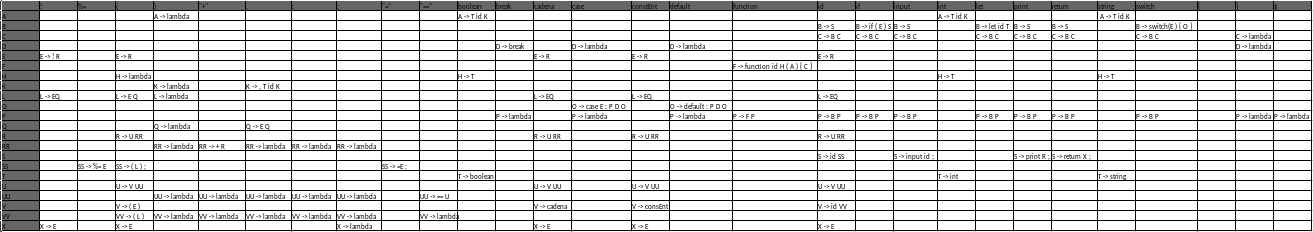
\includegraphics[width=1\textwidth]{tablaM.png}}
\caption{\label{figura:tablaM}Tabla de Análisis de LL1 (Click para una hoja de cálculo con mayor resolución).}
\end{figure}

\newpage
\begin{appendices}

\section{Casos de Prueba}

\subsection{Prueba Funcional 1}
Código fuente:
\lstinputlisting[language=JavaScript]{FicheroFuente1.txt}
\hspace{\parindent} Fichero de Parse y Árbol Sintáctico:
\lstinputlisting[language=JavaScript]{ficheroParse1.txt}
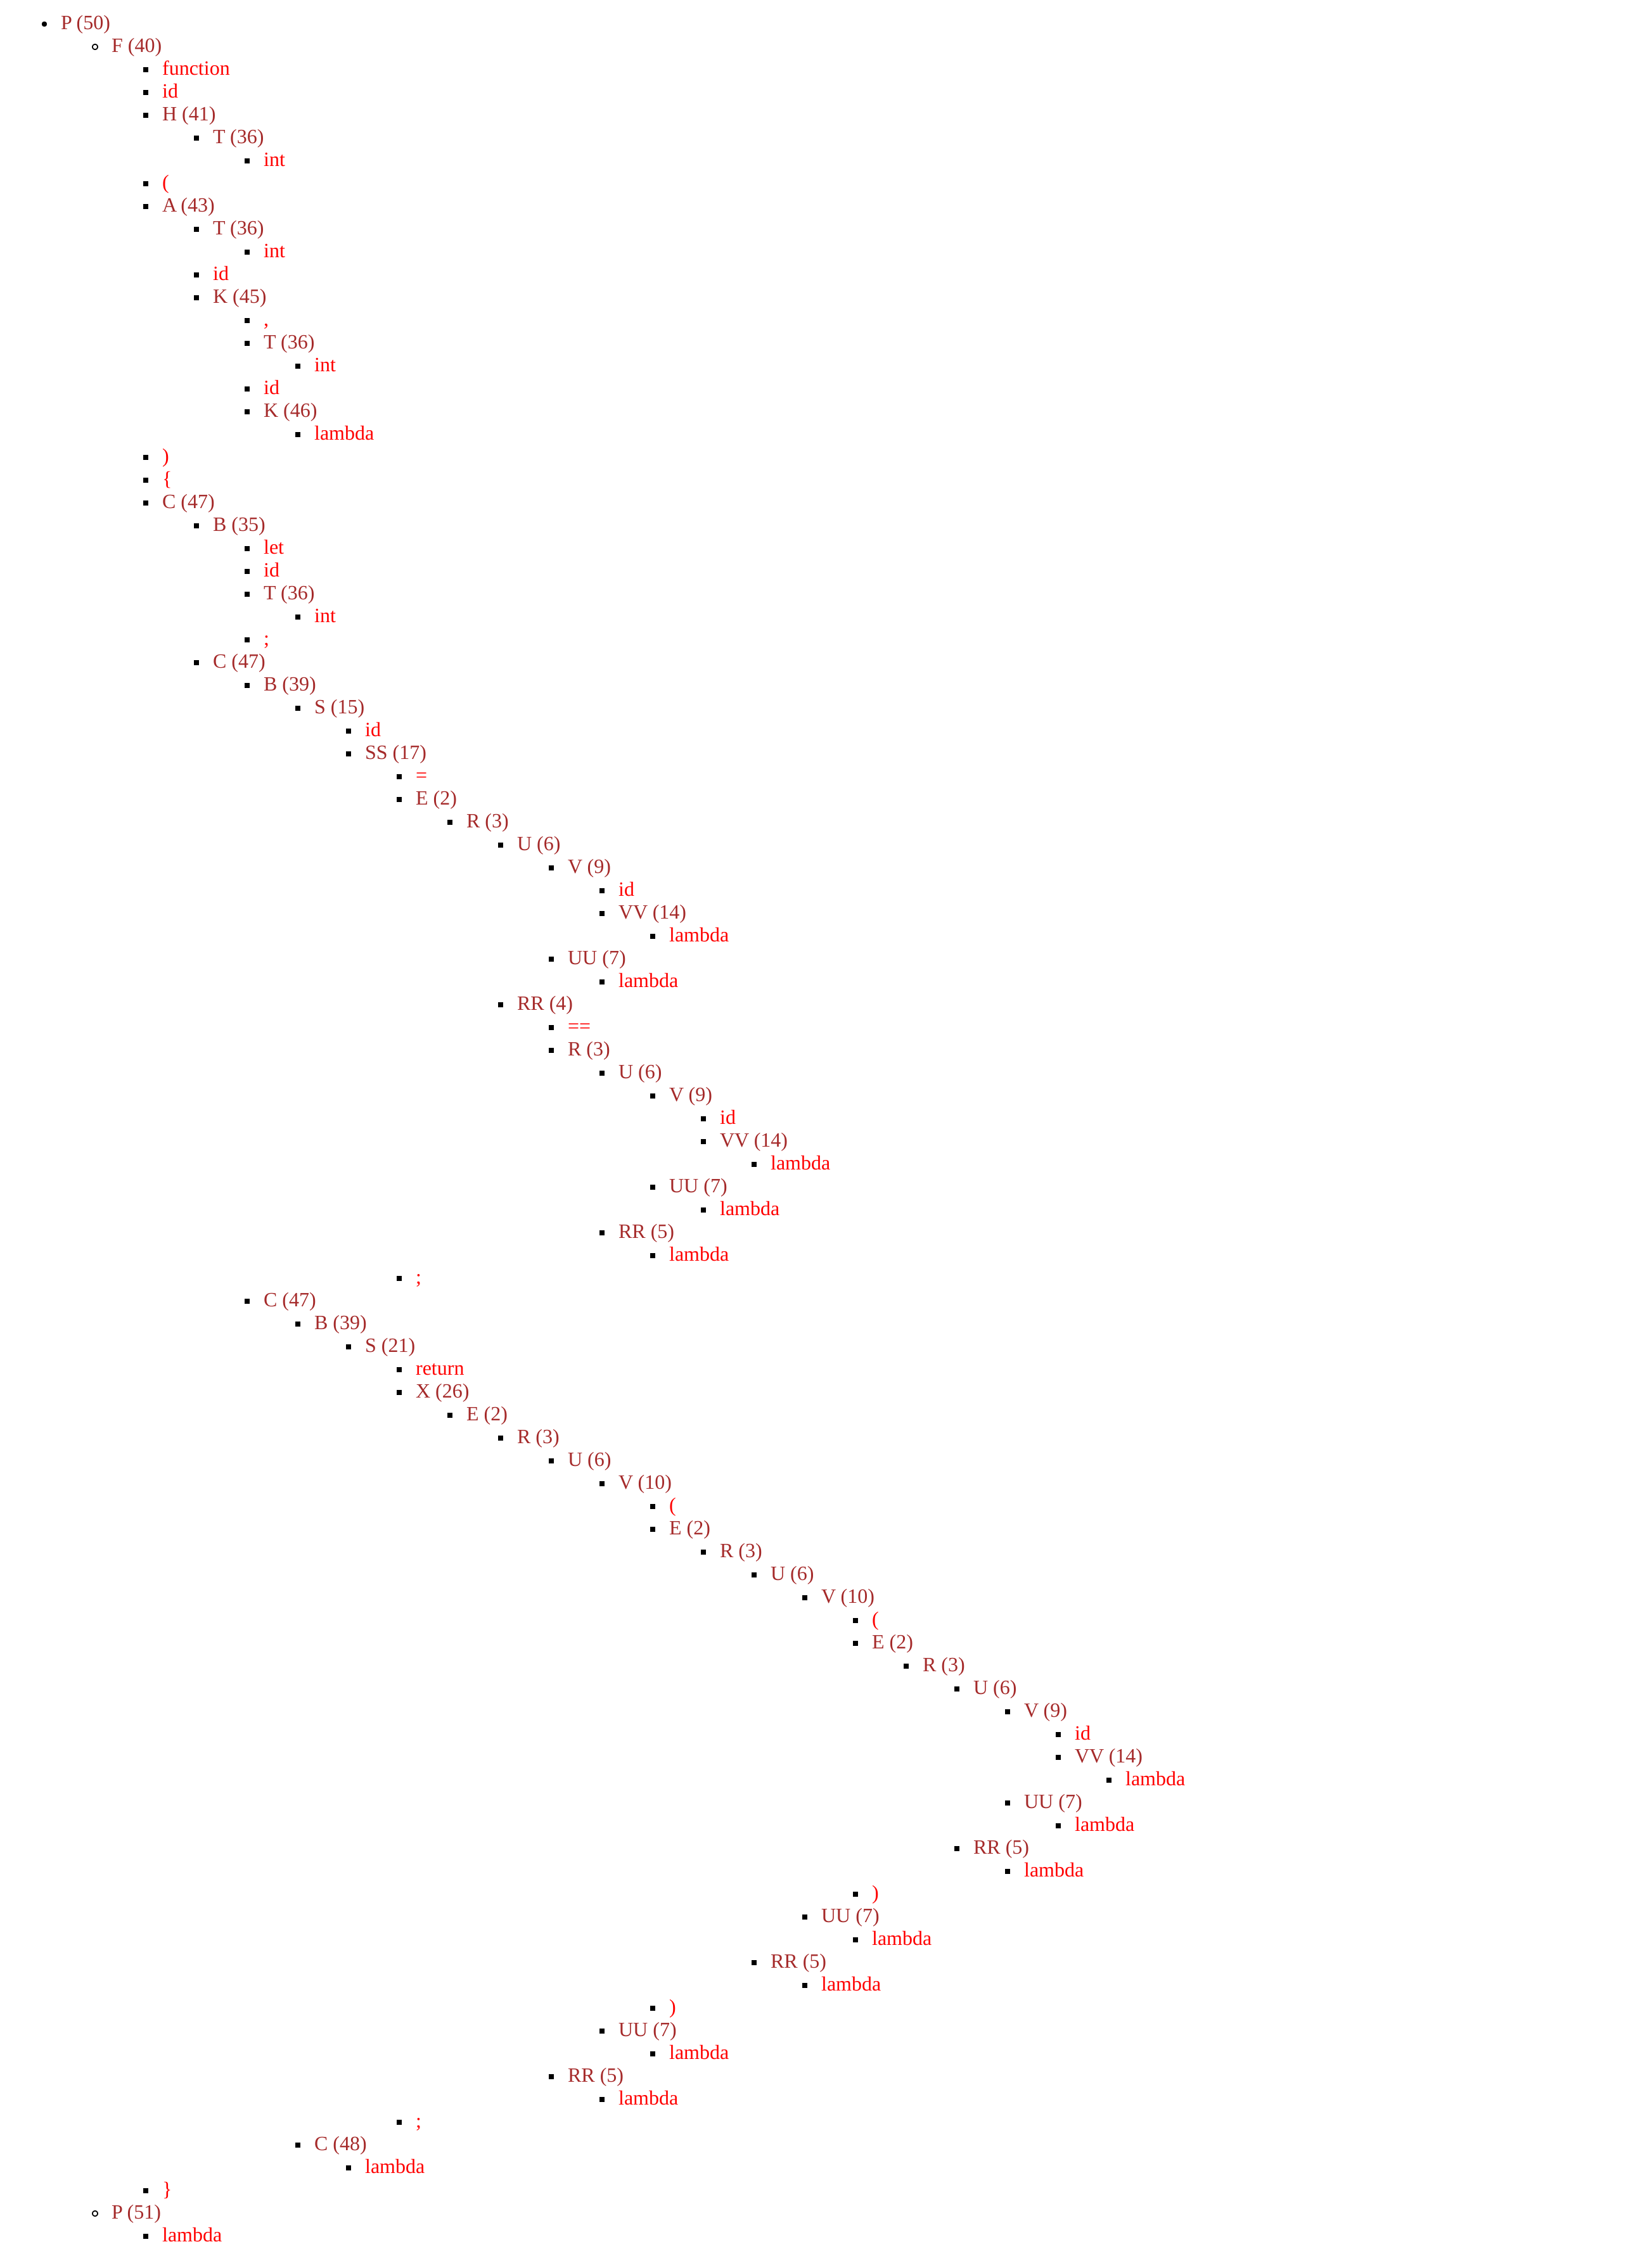
\includegraphics[width=0.7\textwidth]{arbol1.png}

\subsection{Prueba Funcional 2}
Código fuente:
\lstinputlisting[language=JavaScript]{FicheroFuente2.txt}
\hspace{\parindent} Fichero de Parse y Árbol sintáctico:
\lstinputlisting[language=JavaScript]{ficheroParse2.txt}
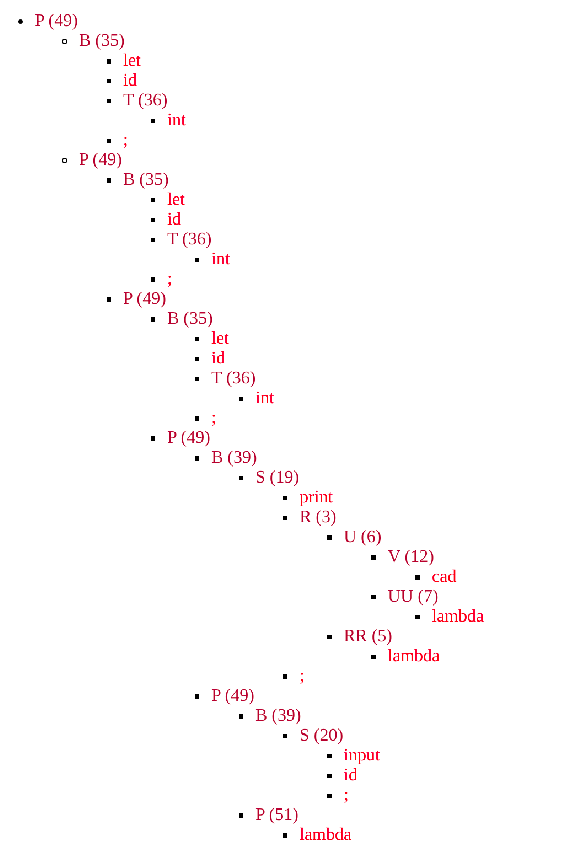
\includegraphics[width=0.5\textwidth]{arbol2.png}

\subsection{Prueba Funcional 3}
Código fuente:
\lstinputlisting[language=JavaScript]{FicheroFuente3.txt}
\hspace{\parindent} Fichero de Parse y Árbol sintáctico:
\lstinputlisting[language=JavaScript]{ficheroParse3.txt}
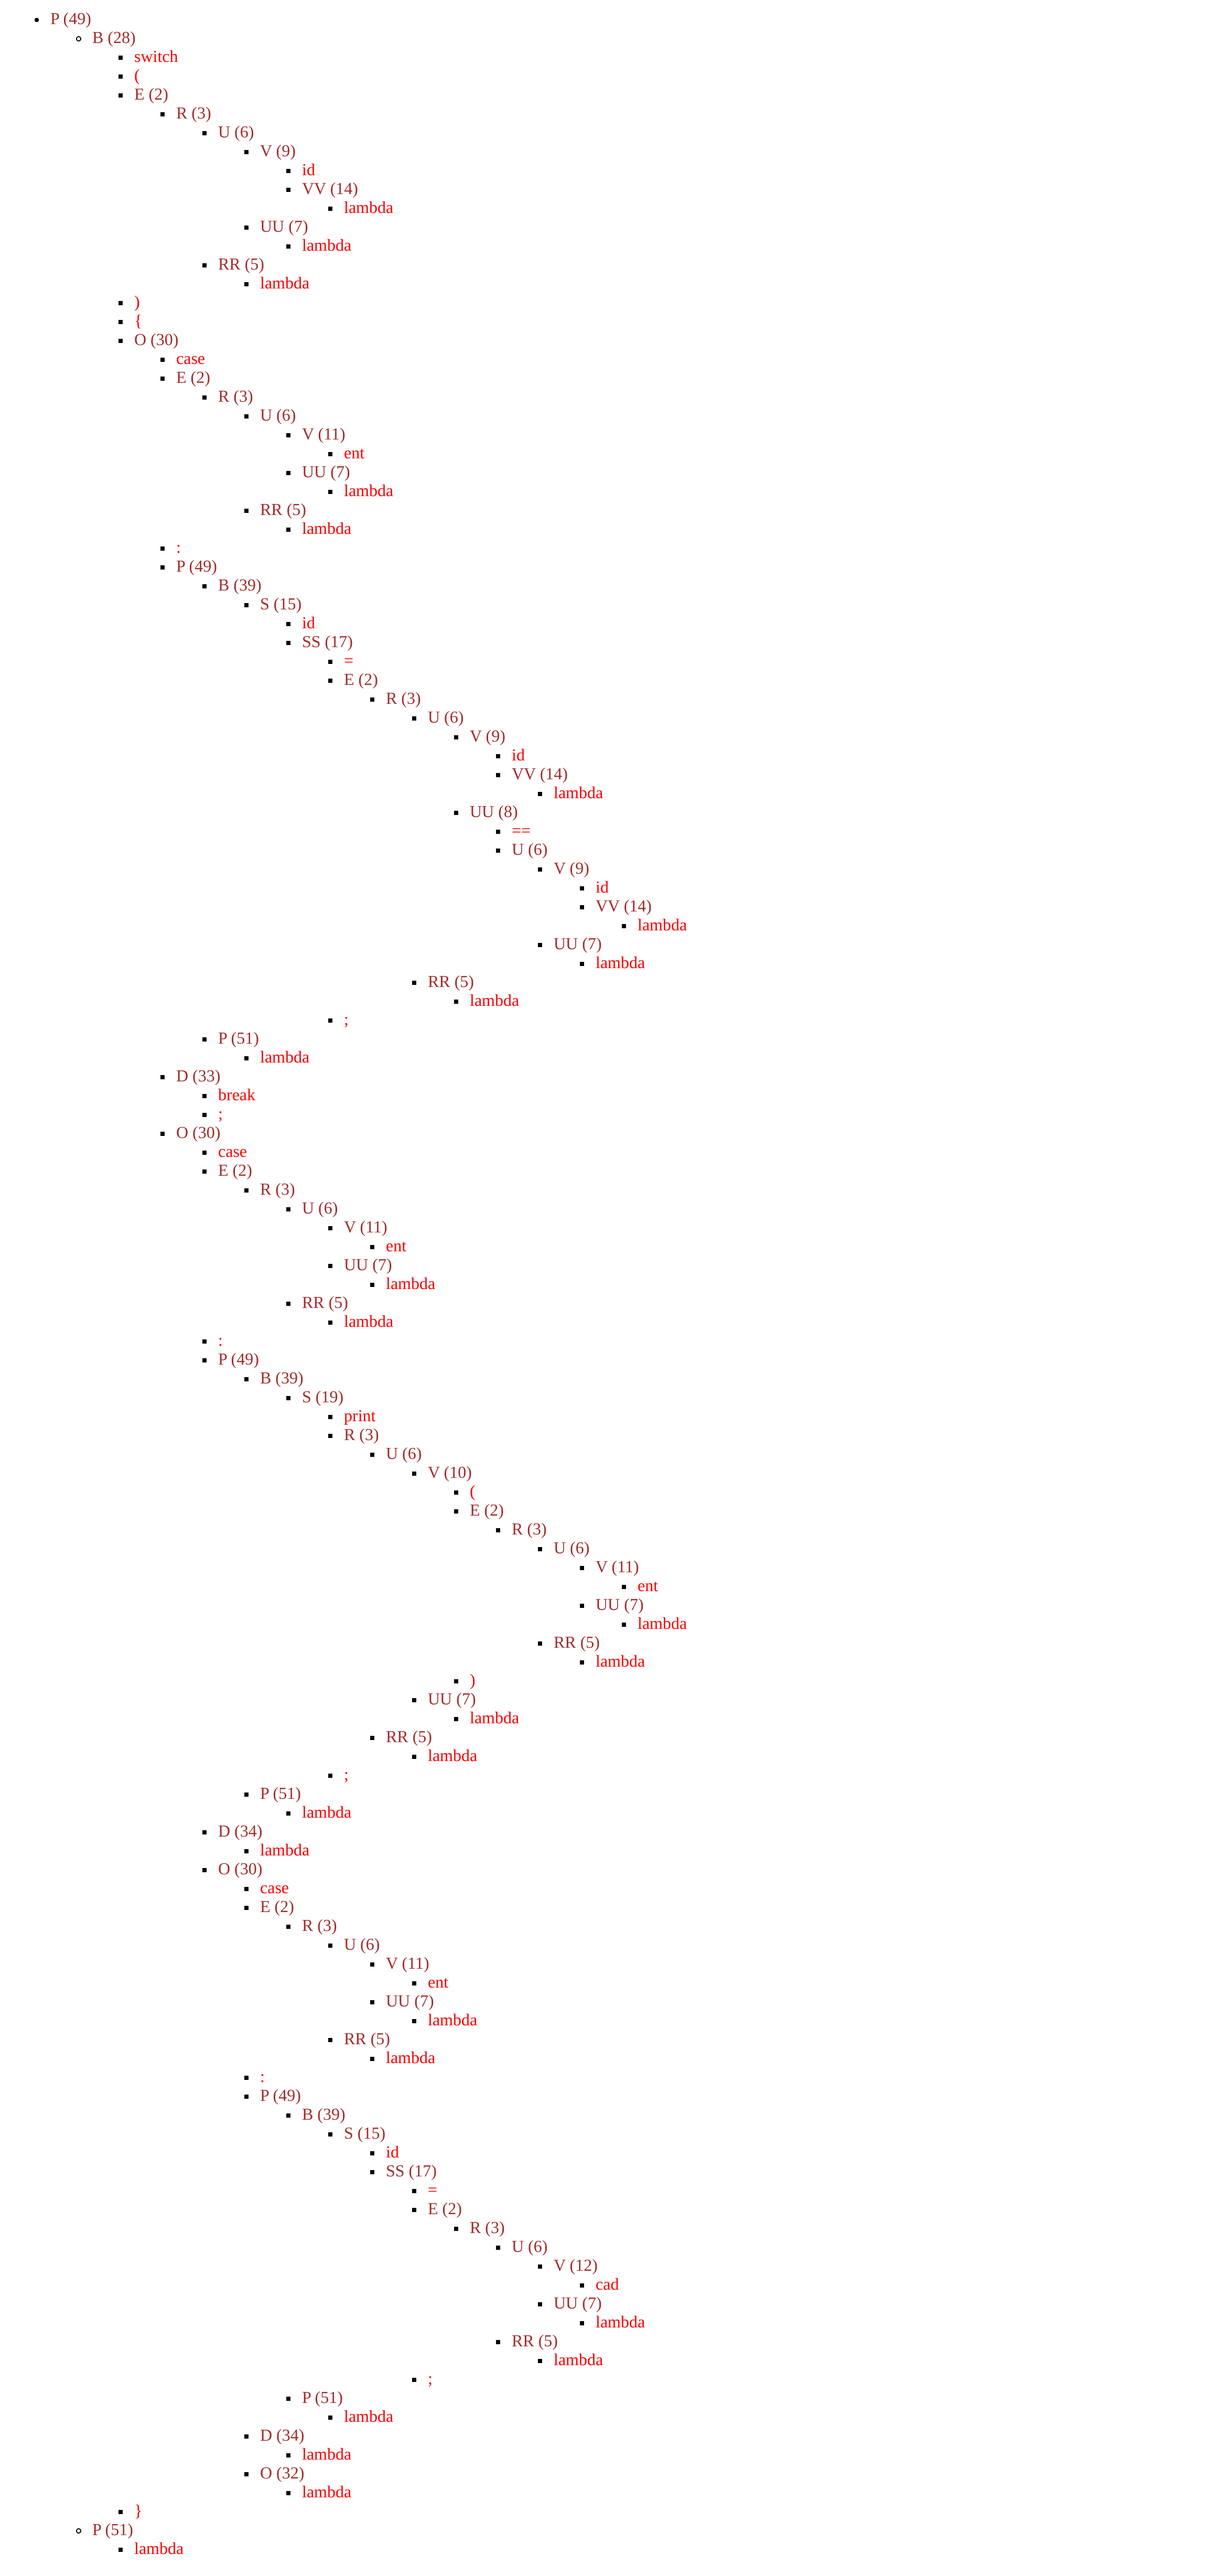
\includegraphics[width=0.65\textwidth]{arbol3.png}

\subsection{Prueba No Funcional 1}
Código fuente:
\lstinputlisting[language=JavaScript]{codigoerror1.txt}
En este caso de prueba vemos que al no poderse declarar una variable dentro de una asignación, a la hora de llegar al apartado de expresiones de la gramática, no existe una regla que permita ir a let, se para la ejecución y imprime por pantalla:\\
\tab \textcolor{red}{Error Sintáctico: No existe regla para M[E, <palabraReservada, let>]}

\subsection{Prueba No Funcional 2}
Código fuente:
\lstinputlisting[language=JavaScript]{codigoerror2.txt}
En este caso de prueba vemos que al no cerrar una llave al acabar el programa, la pila no se vacia al final del programa y finaliza la ejecución.\\
\tab \textcolor{red}{Error Sintáctico: No existe regla para M[C, <\$, >]}

\subsection{Prueba No Funcional 3}
Código fuente:
\lstinputlisting[language=JavaScript]{codigoerror3.txt}
En este caso de prueba vemos que al poner una palabra reservada como nombre de una función envia un error, ya que el token que se esperaba era un id, sin embargo, al recibir el token de palabra reservada, no coincide con el de la cima de la pila y acaba la ejecución.\\
\tab \textcolor{red}{Error Sintáctico: El terminal de la cima de la pila "id" no coincide con el token <palabraReservada, int> enviado por el AnLex}

\end{appendices}

\end{document}
